\documentclass{beamer}
\usetheme{Goettingen}
\usefonttheme{professionalfonts}
\usefonttheme[onlymath]{serif}
\setbeamertemplate{caption}{\insertcaption}

\usepackage[version=4]{mhchem}
\usepackage{graphicx}
\usepackage{svg}
\usepackage{empheq}
\usepackage[many]{tcolorbox}

\usepackage{smartdiagram}
\usepackage{metalogo}
\usepackage{dtklogos}

\usepackage{times}
\usepackage{amsmath}
\usepackage{verbatim}

\usepackage{tikz}
\usetikzlibrary{arrows,shapes,positioning,shadows,trees,matrix,math,calc,mindmap}
\tikzset{>=stealth}
\newcommand{\tikzmark}[3][]{\tikz[remember picture,baseline] \node [anchor=base,#1,](#2) {#3};}
\def\centerarc[#1](#2)(#3:#4:#5){\draw[#1]($(#2)+({#5*cos(#3)},{#5*sin(#3)})$) arc (#3:#4:#5);}

\title[Molecular Hydrophobicity Potential]
{%
    Implementing Molecular Hydrophobicity Potential Measurment for the Analysis of Dynamic Biomolecular Interactions
}
\date{\today}
\author[Pelg Bar Sapir]
{
    Peleg Bar Sapir\inst{1} \and \\ ~\\
    Under supervision of\\Prof. Maria Andrea Mroginski\inst{2}
}
\institute[Freie Universit\"{a}t Berlin, Techniche Universit\"{a} Berlin]
{
    \inst{1}%
        Freie Universit\"{a}t Berlin
    \and
    \vskip-2mm
    \inst{2}%
        Techniche Universit\"{a}t Berlin
}

\begin{document}
\tikzstyle{every picture}+=[remember picture]
\everymath{\displaystyle}

\begin{frame}
    \titlepage
\end{frame}

\begin{frame}{Outline}
	\setcounter{tocdepth}{2}
    \tableofcontents
\end{frame}

\section{Introduction}
\subsection{Hydrophobicity and log P}
\begin{frame}{Hydrophobicity and log P}
	\tikzset{every node/.append style={scale=0.7}, grow cyclic}
    \tikzset{level 1/.append style={sibling angle=50, level distance=250mm}}
    \tikzset{level 2/.append style={sibling angle=20, level distance=125mm}}
	\centering
	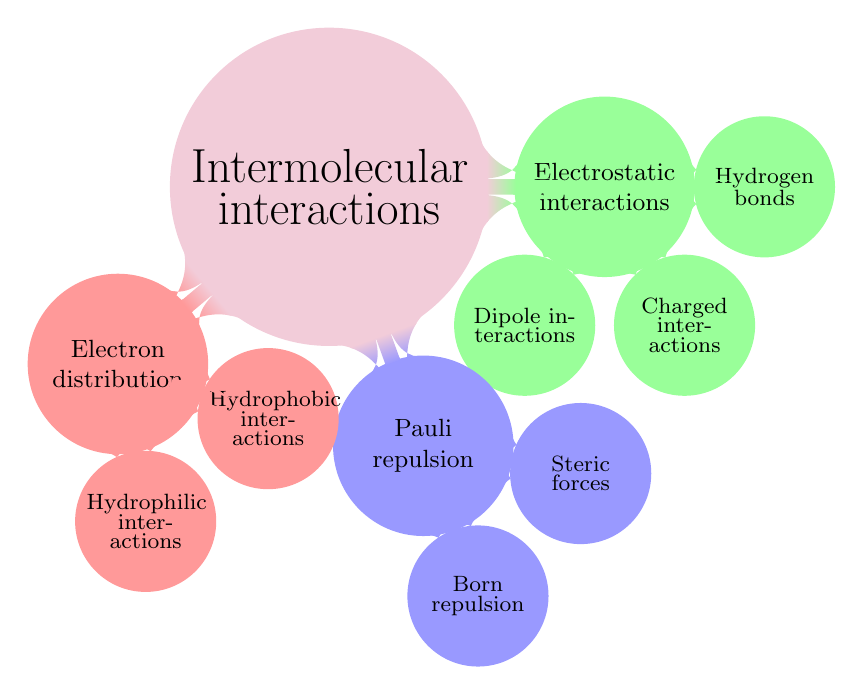
\begin{tikzpicture}[scale=0.7]
		\path[mindmap, concept color=purple!20, text=black]
		node[concept, font=\fontsize{16pt}{15pt}\selectfont] {Intermolecular interactions}
		[clockwise from=0]
		child[concept color=green!40] {
			node[concept] {Electrostatic interactions}
			child { node[concept, font=\fontsize{8pt}{7pt}\selectfont] {Hydrogen bonds} }
			child { node[concept, font=\fontsize{8pt}{7pt}\selectfont] {Charged interactions} }
			child { node[concept, font=\fontsize{8pt}{7pt}\selectfont] {Dipole interactions} }
		}
		child[concept color=blue!40, rotate=-10] {
			node[concept] {Pauli repulsion}
			child { node[concept, font=\fontsize{8pt}{7pt}\selectfont] {Steric forces} }
			child { node[concept, font=\fontsize{8pt}{7pt}\selectfont] {Born repulsion} }
		}
		child[concept color=red!40, rotate=-20] {
			node[concept] {Electron distribution}
			child { node[concept, font=\fontsize{8pt}{7pt}\selectfont] {Hydrophobic interactions} }
			child { node[concept, font=\fontsize{8pt}{7pt}\selectfont] {Hydrophilic interactions} }
		};
	\end{tikzpicture}
\end{frame}

\begin{frame}{Hydrophilic/Hydrophobic Interactions}
\end{frame}

\subsection{Partition Coefficient}
\begin{frame}{Partition Coefficient}
	\centering
	\begin{tcolorbox}[colback=blue!5, colframe=blue!40!black, title=Definition]
		The ratio of concentrations of a compound in a mixture of two immiscible phases at equilibrium
	\end{tcolorbox}
	\begin{itemize}
        \setlength\itemsep{1.5em}
		\uncover<2->{\item Commonly used: water and octanol}
		\uncover<3->{\item Can be measured at an \alert{ionized} or \alert{unionized} state}
		\uncover<4->{\item $\log P_{\text{octanol/water}}=\log\left(\frac{\left[\text{solute}\right]_{\text{water}}}{\left[\text{solute}\right]_{\text{octanol}}}\right)$}
		\uncover<5->{\item Hydrophobicity \alert{increases} with the (common) $\log P$}
	\end{itemize}
\end{frame}

\section{Molecular Hydrophobicity Potential}
\subsection{What is it?}
\begin{frame}{What is Molecular Hydrophobicity Potential (MHP)?}
	\begin{itemize}
        \setlength\itemsep{1.5em}
		\uncover<1->{\item By measuring the $\log P$ of many (ca. 30,000) compounds\footnote{Ghose et al, J. Phys. Chem. A 1998, 102, 3762-3772}, single atoms can be assigned local "force" values.}
		\uncover<2->{\item Combining these values with a distance-depended decay function, a potential can be constructed.}
		\uncover<3->{\item This potential predicts the local $\log P$ behaviour of fragments of a molecule.}
	\end{itemize}
\end{frame}

\subsection{Potential}
\subsubsection{General form}

\begin{frame}{The MHP Formula}
    \centering
    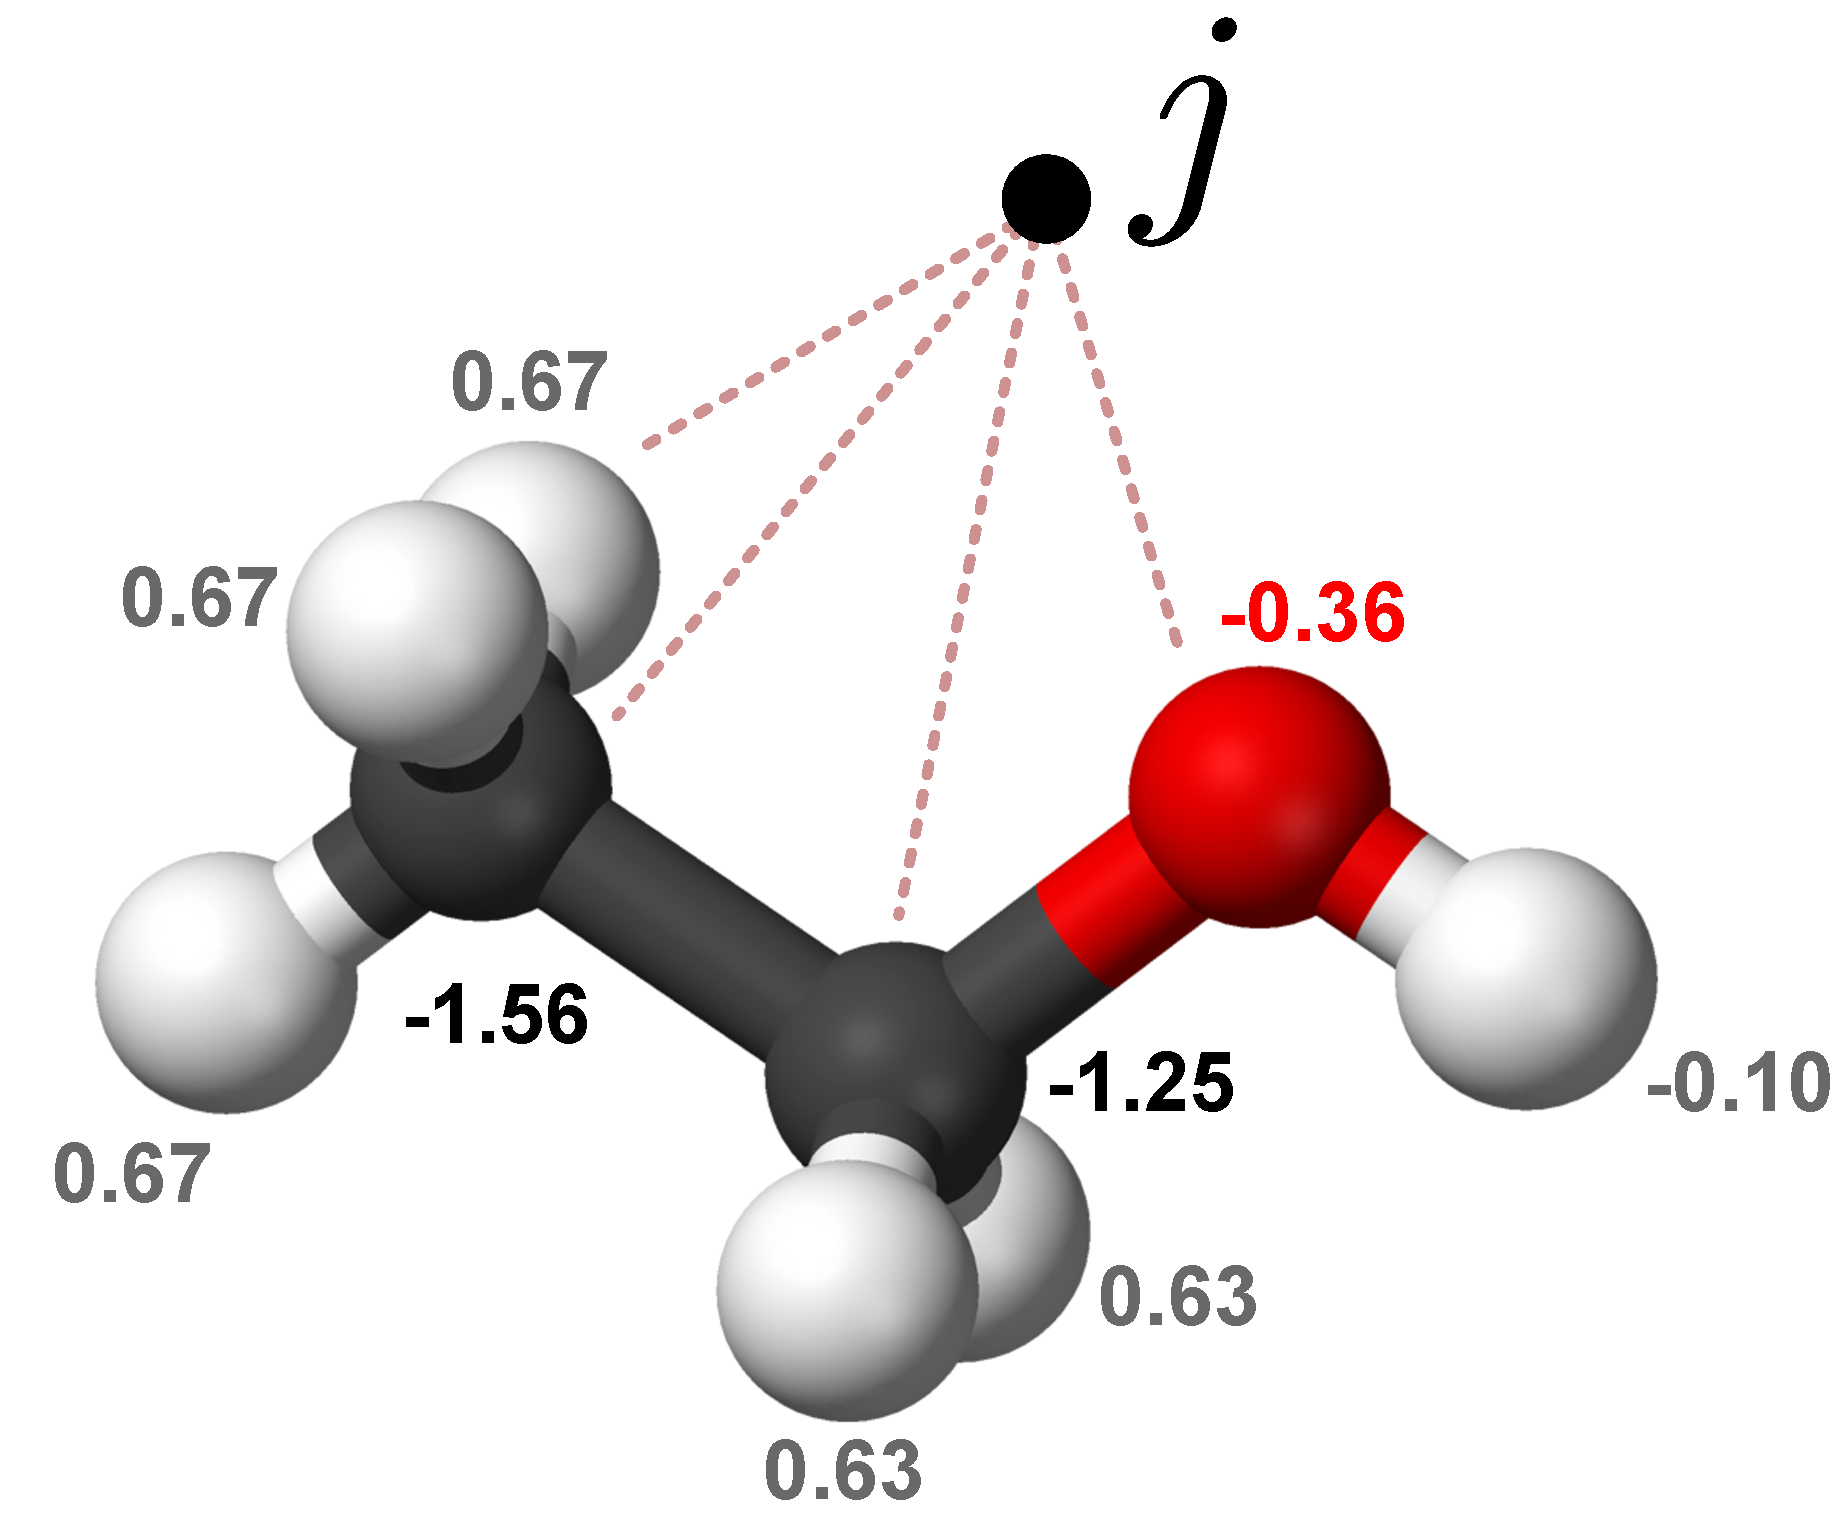
\includegraphics[scale=0.125]{mhp_visual1.eps}

    \begin{equation*}
        \text{MHP}\left(\mathbf{x'}\right)=
        \tikz[baseline]{
            \node[anchor=base] (sum)
            {$\sum_{i=1}^{k}\limits$};
        }\left[ 
        \tikz[baseline]{
            \node[anchor=base] (force)
            {$f_i$};
        } \cdot
        \tikz[baseline]{
            \node[anchor=base] (distance)
            {$D\left(\mathbf{x}-\mathbf{x'}_i\right)$};
        }\right]
    \end{equation*}

    \begin{tikzpicture}[overlay, remember picture,node distance=1.5cm]
        \uncover<2->{\node[fill=blue!20, xshift=1.2cm, yshift=0.5cm] (sumdescr) [below left=of sum]{Summing over all atoms};}
        \uncover<2->{\draw[->,thick] (sumdescr) to [in=-90,out=90] (sum);}
        \uncover<2->{\node[fill=blue!20] at (sum) {$\sum_{i=1}^{k}\limits$};}
                        
        \uncover<3->{\node[fill=red!20, yshift=-0.2cm] (forcedescr) [below = of force]{Force constants};}
        \uncover<3->{\draw[->,thick] (forcedescr) to [in=-90,out=90] (force);}
        \uncover<3->{\node[fill=red!20] at (force) {$f_i$};}

        \uncover<4->{\node[fill=green!20, xshift=-2.0cm,yshift=0.5cm] (distancedescr) [below right = of distance]{Distance function};}
		\uncover<4->{\draw[->,thick] (distancedescr) to [in=-90,out=90] (distance.south);}
        \uncover<4->{\node[fill=green!20] at (distance) {$D\left(\mathbf{x}-\mathbf{x'}_i\right)$};}
	\end{tikzpicture}
\end{frame}

\subsubsection{Force Constants}
\begin{frame}{Force Constants - Carbon}
    \centering
        \begin{table}[H]
            \caption{\textbf{Carbon} atom contribution to hydrophobicity\footnote{Source: Ghose et al, J. Phys. Chem. A 1998, 102, 3762-3772}}
            \begin{tabular}{l l r}
                Type & Description & $f_i$ value \\
                \hline
                & \underline{Carbon in:} &         \\
                1   & $\ce{CH_{3}R}$     & -1.5603 \\
                3   & $\ce{CHR_{3}}$     & -0.6681 \\
                7   & $\ce{CH_{2}X_{2}}$ & -1.0305 \\
                13  & $\ce{RCX_{3}}$     &  0.7894 \\
                17  & $\ce{=CR_{2}}$     &  0.0383 \\
                24  & $\ce{R--CH--R}$    & -0.3251 \\
                25  & $\ce{R--CR--R}$    &  0.1492 \\
                26  & $\ce{R--CX--R}$    &  0.1539 \\
                \hline
            \end{tabular}
        \end{table}
\end{frame}
\begin{frame}{Force Constants - Hydrogen}
    \centering
        \begin{table}[H]
            \caption{\textbf{Hydrogen} atom contribution to hydrophobicity\footnote{Source: Ghose et al, J. Phys. Chem. A 1998, 102, 3762-3772}}
            \begin{tabular}{l l r}
                Type & Description & $f_i$ value \\
                \hline
                & \underline{Hydrogen attached to}:              &         \\
                46  & $\ce{C_{sp^{3}}}$, no $\ce{X}$ in $\alpha$ &  0.7341 \\
                47  & $\ce{C_{sp^{2}}}$                          &  0.6301 \\
                50  & Heteroatom $\ce{X}$                        & -0.1036 \\
                52  & $\ce{C_{sp^{3}}}$, 1 $\ce{X}$ in $\alpha$  &  0.6666 \\
                54  & $\ce{C_{sp^{3}}}$, 3 $\ce{X}$ in $\alpha$  &  0.6338 \\
                \hline
            \end{tabular}
        \end{table}
\end{frame}
\begin{frame}{Force Constants - Oxygen}
    \centering
        \begin{table}[H]
            \caption{\textbf{Oxygen} atom contribution to hydrophobicity\footnote{Source: Ghose et al, J. Phys. Chem. A 1998, 102, 3762-3772}}
            \begin{tabular}{l l r}
                Type & Description & $f_i$ value \\
                \hline
                    & \underline{Oxygen in}:           &         \\
                56  & Alcohol                          & -0.3567 \\
                57  & Phenol, enol, carboxyl $\ce{OH}$ & -0.0127 \\
                58  & Ketone                           & -0.0233 \\
                61  & Nitro, N-oxides                  &  1.0520 \\
                62  & $\ce{O-}$                        & -0.7941 \\
                \hline
            \end{tabular}
        \end{table}
\end{frame}
\begin{frame}{Force Constants - Various}
    \centering
        \begin{table}[H]
            \caption{\textbf{Various} atom contribution to hydrophobicity\footnote{Source: Ghose et al, J. Phys. Chem. A 1998, 102, 3762-3772}}
            \begin{tabular}{l l r}
                Type & Description & $f_i$ value \\
                \hline
                66   & $\ce{N}$ in Primary amine              & -0.5427 \\
                67   & $\ce{N}$ in Secondary amine            & -0.3168 \\
                81   & $\ce{F}$ attached to $\ce{C_{sp^{3}}}$ &  0.4797 \\
                106  & $\ce{S}$ in $\ce{R-SH}$   (thiol)      &  1.0520 \\
                119  & $\ce{P}$ in $\ce{PR_{3}}$ (phosphine)  & -0.7941 \\
                \hline
            \end{tabular}
        \end{table}
\end{frame}

\subsubsection{Distance function}
\begin{frame}{Distance function}
    \centering
    \begin{minipage}[t]{0.48\linewidth}
        \centering
        Audry form
        \begin{empheq}[box=\tcbhighmath]{align*}
            D\left(x\right)=\frac{1}{1+x}
        \end{empheq}
    \end{minipage}
    \begin{minipage}[t]{0.48\linewidth}
        \centering
        Exponential decay form
        \begin{empheq}[box=\tcbhighmath]{align*}
            D\left(x\right)=e^{-\alpha x}
        \end{empheq}
    \end{minipage}
    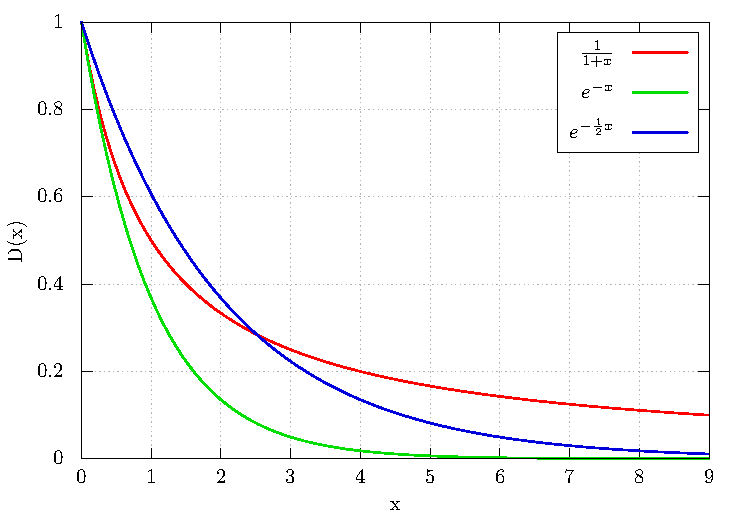
\includegraphics[scale=0.65]{dist_funcs.pdf}    
\end{frame}

\subsection{Surface}
\subsubsection{Solvent Accesible Surface}
\begin{frame}{Solvent Accesible Surface}
    \begin{itemize}
        \uncover<1->{\item The surface around a molecule accesible to solvent molecules}
        \uncover<2->{\item[] \centering
            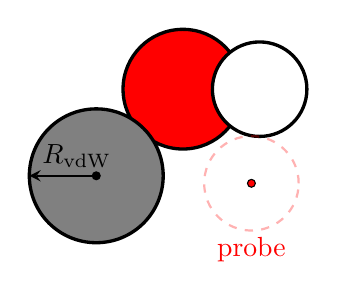
\begin{tikzpicture}[scale=0.5]
                % Scale, distances, coordinates and radii
                \def\scal{1.0}
                \def\dOH{1.95*\scal}
                \def\dOC{2.20*\scal}
                \def\RP{1.20*\scal}
                \coordinate (O) at (2.30,6.70);
                \def\RO{1.52*\scal}
                \def\ROP{\RO+\RP}	
                \coordinate (H) at ($(O)+(\dOH,0)$);
                \def\RH{1.20*\scal}
                \def\RHP{\RH+\RP}	
                \coordinate (C) at ($(O)-(\dOC,\dOC)$);
                \def\RC{1.70*\scal}
                \def\RCP{\RC+\RP}
                \pgfmathsetmacro\pang{-95}
                \pgfmathsetmacro\Px{cos(\pang)*(\RH+\RP)}
                \pgfmathsetmacro\Py{sin(\pang)*(\RH+\RP)}


                % Cut radii+probe (should be parameterized...)
                \centerarc[thick, fill=blue!10, dashed](O)(0:365:2.72);
                \centerarc[thick, fill=blue!10, dashed](H)(-105:105:2.4);
                \centerarc[thick, fill=blue!10, dashed](C)(98:352:2.9);

                % Atoms	
                \filldraw[very thick, fill=red]
                (O) circle[radius=\RO];
                \filldraw[very thick, fill=white]
                (H) circle[radius=\RH];
                \filldraw[very thick, fill=gray]
                (C) circle[radius=\RC];
                \draw[->, thick] (C) --++(-\RC,0);
                \filldraw[fill=black] (C) circle (0.1);
                \node[] at ($(C)+(-.5,.5)$) {$R_{\text{vdW}}$};
                \draw[thick, opacity=0.3, red, dashed] ($(H) + (\Px,\Py)$) circle (\RP);
                \filldraw[fill=red] ($(H) + (\Px,\Py)$) circle (0.1);
                \node[red] at ($(H) + (\Px,1.7*\Py)$) {probe};
            \end{tikzpicture}
            }
        \uncover<3->{\item[] (For water molecules usually $r=1.4\left[\text{\AA}\right]$)}
    \end{itemize}
\end{frame}

\begin{frame}{How to Create the Solvent Accesible Surface?}
	\centering
	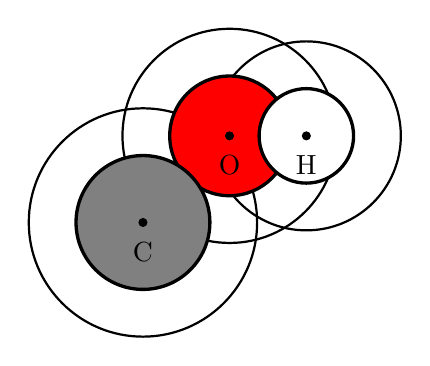
\begin{tikzpicture}[scale=.5]
        % Scale, distances, coordinates and radii
        \def\scal{1.0}
        \def\dOH{1.95*\scal}
        \def\dOC{2.20*\scal}
        \def\RP{1.20*\scal}
        \coordinate (O) at (2.30,6.70);
        \def\RO{1.52*\scal}
        \def\ROP{\RO+\RP}	
        \coordinate (H) at ($(O)+(\dOH,0)$);
        \def\RH{1.20*\scal}
        \def\RHP{\RH+\RP}	
        \coordinate (C) at ($(O)-(\dOC,\dOC)$);
        \def\RC{1.70*\scal}
        \def\RCP{\RC+\RP}
	
		% Full radii+probe	
		\uncover<5-8>{\draw[thick]
				      (O) circle[radius=\ROP];}
		\uncover<6-8>{\draw[thick]
				      (H) circle[radius=\RHP];}
		\uncover<7-8>{\draw[thick]
					  (C) circle[radius=\RCP];}

		% Cut radii+probe (should be parameterized...)
		\uncover<9- >{\centerarc[thick, fill=white](O)(0:365:2.72);}
		\uncover<8-8>{\centerarc[thick, red](O)(-58:60:2.72);}
		\uncover<8-8>{\centerarc[thick, red](O)(165:283:2.72);}
		\uncover<9- >{\centerarc[thick, fill=white](H)(-105:105:2.4);}
		\uncover<8-8>{\centerarc[thick, red](H)(105:255:2.4);}
		\uncover<9- >{\centerarc[thick, fill=white](C)(98:352:2.9);}
		\uncover<8-8>{\centerarc[thick, red](C)(-8:98:2.9);}

		% Atoms	
		\uncover<3->{\filldraw[very thick, fill=red]
		(O) circle[radius=\RO];}
		\uncover<3->{\filldraw[very thick, fill=white]
		(H) circle[radius=\RH];}
		\uncover<3->{\filldraw[very thick, fill=gray]
		(C) circle[radius=\RC];}
		
		% Points
		\uncover<1-2>{\coordinate (DV) at (0,0.75);}
		\uncover<1-2>{\node[] at ($(O)-(DV)$) {O};}
		\uncover<1-2>{\filldraw[black] (O) circle [radius=0.1];}
		\uncover<1-2>{\node[] at ($(H)-(DV)$) {H};}
		\uncover<1-2>{\filldraw[black] (H) circle [radius=0.1];}
		\uncover<1-2>{\node[] at ($(C)-(DV)$) {C};}
		\uncover<1-2>{\filldraw[black] (C) circle [radius=0.1];}
	\end{tikzpicture}
	
	\begin{enumerate}
		\uncover<2->{\item Take all atoms with their vdW-radii}
		\uncover<4->{\item Create spheres around all atoms with $R^{i}=R^{i}_{\text{vdw}}+R_{\text{probe}}$}
		\uncover<8->{\item Delete all points that are "burried" in other extended spheres
			  (i.e. $\Delta\left(p^{i},c^{j}\right)\leq R^{j}+R_{\text{probe}}$)}
		\uncover<9->{\item The remaining surface is the solvent-accesible surface of the molecule}
	\end{enumerate}
\end{frame}

\subsubsection{Evenly Distributed Points}
\begin{frame}{Evenly Distributed Points}
    \centering
    How to distribute $N$ points on a surface of a sphere?\\ ~\\ ~\\
    \begin{columns}
        \uncover<1->{
        \begin{column}{0.4\textwidth}
        \centering
	        \includesvg[scale=.17]{sphere_wireframe_coords}\\
        \end{column}
        }
        
        \uncover<3->{
        \begin{column}{0.2\textwidth}
        \centering
	        \includesvg[scale=.17]{arrow_right}
        \end{column}
        \begin{column}{0.4\textwidth}
        \centering
	        \includesvg[scale=.17]{sphere_wireframe_points}
        \end{column}
    }
    \end{columns}
    \begin{columns}
        \begin{column}{0.4\textwidth}
            \begin{itemize}
                \uncover<2->{\item[] $\varphi_{i}=i\cdot\frac{2\pi}{N}$}
                \uncover<2->{\item[] $\theta_{j}=j\cdot\frac{\pi}{N}$}
            \end{itemize}
        \end{column}
        \begin{column}{0.2\textwidth}
        \end{column}
        \begin{column}{0.4\textwidth}
            \begin{itemize}
                \uncover<4->{\item Points are not evenly distributed}
                \uncover<5->{\item Several points overlap at poles}
            \end{itemize}
        \end{column}
    \end{columns}
\end{frame}

\begin{frame}{Evenly Distributed Points}
    \centering
    Solution: \alert{Vogel's method}\\
    \begin{columns}
        \begin{column}{0.5\textwidth}
            \uncover<1->{In 2 dimensions:}
            \begin{itemize}
                \uncover<2->{\item Distances: $r_{i}=\sqrt{\frac{i}{N}}$}
                \uncover<2->{\item Angle: $\theta_{i}=\varphi i$
                			 \item[] ($\varphi$ is the golden ratio!)}
            \end{itemize}
        \end{column}
        \begin{column}{0.5\textwidth}
			\centering
			\uncover<3->{\includesvg[scale=0.35]{vogels}}
        \end{column}
    \end{columns}
    ~\\ ~\\
    \begin{columns}
        \begin{column}{0.5\textwidth}
            \uncover<4->{In 3 dimensions (cylindrical coordinates):}
            \begin{itemize}
                \uncover<5->{\item Distances: $z_{i}=\left(1-\frac{1}{N}\right)\left(1-\frac{2i}{N-1}\right)$}
                \uncover<5->{\item Angles: $\theta_{i}=\varphi i,\ \rho_{i}=\sqrt{1-z_{i}^{2}}$}
            \end{itemize}
        \end{column}
        \begin{column}{0.5\textwidth}
			\centering
			\uncover<6->{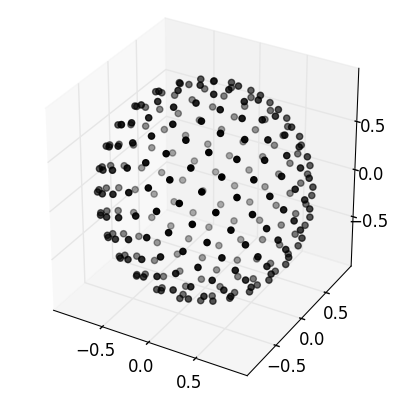
\includegraphics[scale=.4]{3d_vogels.png}\\
                         \tiny{Image source: Marmakoide's Blog}
            }
        \end{column}
    \end{columns}
\end{frame}

\subsubsection{Integration}
\begin{frame}{Integration}
    \begin{itemize}
        \setlength\itemsep{1.5em}
        \uncover<1->{\item Each atom's total surface area: $V^{a}=4\pi\left(R_{\text{vdW}}^{a}+R_{\text{probe}}\right)^{2}$}
        \uncover<2->{\item The surface is represented by $N$ points}
        \uncover<3->{\item Meaning: each point has $V_{j}^{a}=\frac{4\pi}{N}\left(R_{\text{vdW}}^{i}+R_{\text{probe}}\right)^{2}$}
        \uncover<4->{\item In addition, each point has: $\text{MHP}_{j}^{a}$}
    \end{itemize}
    \centering
    \uncover<5->{
        ~\\Therefore, each atom has a total MHP of:~\\~\\
        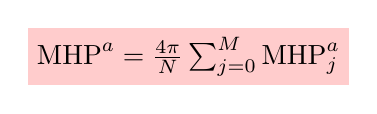
\begin{tikzpicture}
            \node[fill=red!20] at (0,0) {$\text{MHP}^{a}=\frac{4\pi}{N}\sum_{j=0}^{M}\text{MHP}_{j}^{a}$};
        \end{tikzpicture}
    }
\end{frame}

\section{Program}
\subsection{What are we interested in?}
\subsection{Program Specifications}
\begin{frame}{Program Specifications}
    \begin{itemize}
        \setlength\itemsep{1.5em}
        \uncover<1->{\item Written in \textbf{Python3}, utylizing \textbf{ProDy}}
        \uncover<2->{\item Heavy calculation written in \textbf{Cython}}
        \uncover<3->{\item Uses neighbor cells implementation for faster calculation}
        \uncover<4->{\item Uses PSF, PDB and DCD files}
        \uncover<5->{\item Generates a PDB output, MHP values in \textbf{beta} column}
    \end{itemize}
\end{frame}

\begin{frame}{Program Options}
    \begin{itemize}
        \setlength\itemsep{1.5em}
        \uncover<1->{\item Input: PSF + PDB or DCD}
        \uncover<2->{\item Subselection (optional): Atomic selection (like vmd)}
        \uncover<3->{\item Number of points per atom (default: $64$)}
        \uncover<4->{\item Solvent probe radius (defalt: $1.4\AA$)}
        \uncover<5->{\item Cutoff distance for distance function (default: $4\AA$)}
        \uncover<6->{\item Frame range (if DCD)}
    \end{itemize}
\end{frame}

\section{Results}
\subsection{Validation via Known log p Values}
\begin{frame}{Validation via Known $\log P$ Values}
	\begin{itemize}
        \setlength\itemsep{1.5em}
		\uncover<2->{\item By integrating and comparing to known $\log P$ values, a correlation can be measured.}
		\uncover<3->{\item A groups of amino acids of varying hydrophobicity where simulated and their MHP calculated.}
	\end{itemize}
\end{frame}
\begin{frame}{Validation via Known $\log P$ Values}
	\centering
	\begin{figure}[h!]
		\caption{Validation in vacuum (5 frames per molecule)\footnote{MD simulation using NAMD, performed by Dr. Tillmann Utesch}, $R^{2}=0.668$}
		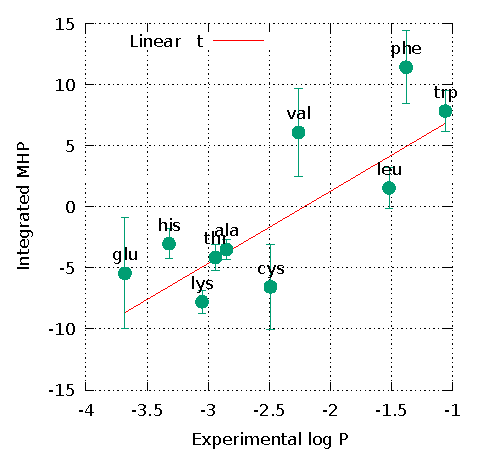
\includegraphics[scale=0.75]{graph_zwitterions_vacuum.eps}
	\end{figure}
\end{frame}
\begin{frame}{Validation via Known $\log P$ Values}
	\centering
	\begin{figure}[h!]
		\caption{Validation in water + structural optimization (10 frames per molecule), $R^{2}=0.748$}
		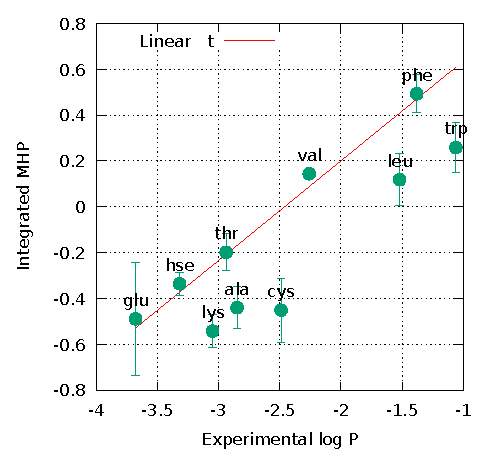
\includegraphics[scale=0.75]{graph_zwitterions_water.eps}
	\end{figure}
\end{frame}
\begin{frame}{Validation via Known $\log P$ Values}
	\centering
	\begin{figure}[h!]
		\caption{Validation in water + structural optimization + SAS normalization (10 frames per molecule), $R^{2}=0.760$}
		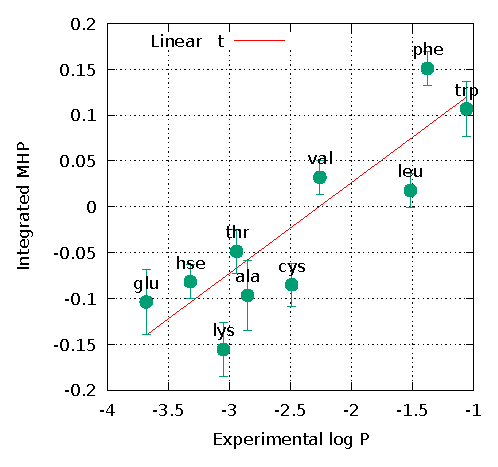
\includegraphics[scale=0.75]{graph_zwitterions_normalized.eps}
	\end{figure}
\end{frame}
\begin{frame}{Validation via Known $\log P$ Values}
	\begin{itemize}
        \setlength\itemsep{1.5em}
		\uncover<2->{\item The validation shows a reasonable qualitative correlation to real data.}
		\uncover<3->{\item Performed in water (with structural optimization), the results became more accurate.}
		\uncover<4->{\item The environment did not match experiments, which could affect the accuracy.}
		\uncover<5->{\item Amino acids are small molecules, each error becomes more significant.}
		\uncover<6->{\item Larger trajectories will sample conformational space better.}
	\end{itemize}
\end{frame}

\subsection{An Example System}
\begin{frame}{An Example System}
	An existing trajectory (100 frames) of a protein-membrane system\footnote{Trajectory provided by Dr. Alejandra de Miguel Catalina} was analazyed.\\
	\begin{itemize}
        \setlength\itemsep{1.5em}
		\uncover<1->{\item The peptide: OP-145, a Cathelicidin derivative with improved properties.}
		\uncover<2->{\item The interaction mechanism pathway was studied by means of all-atom simulation.}
		\uncover<3->{\item The membrane used for the study consists of a mixture of two lipids, PG and PE, in agreement with experimental measurements.}
	\end{itemize}
\end{frame}
\begin{frame}{A video of the system}
\end{frame}
\begin{frame}{MHP Change Over Time}
	\centering
	\begin{figure}[h!]
		\caption{MHP change over time for ARG-7}
		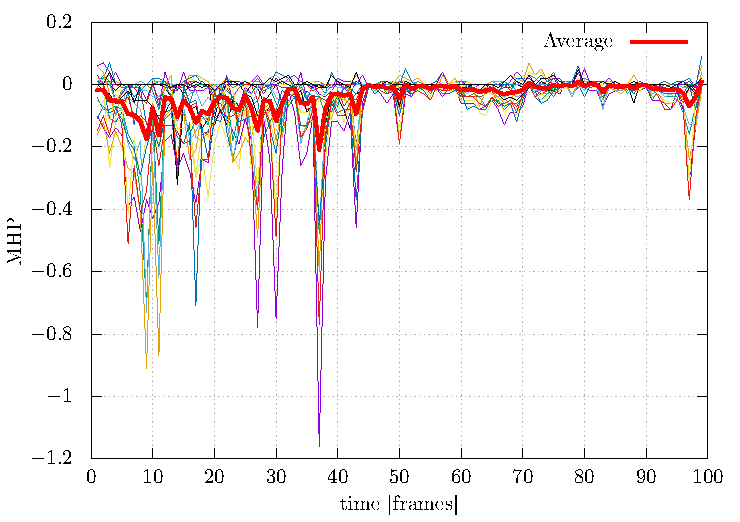
\includegraphics[scale=0.75]{ARG07_graph.pdf}
	\end{figure}
\end{frame}
\begin{frame}{MHP Change Over Time}
	\centering
	\begin{figure}[h!]
		\caption{MHP change over time for ARG-24}
		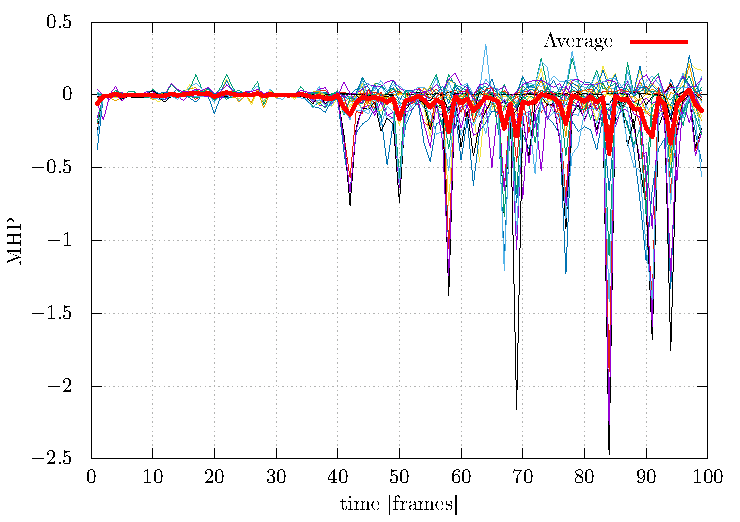
\includegraphics[scale=0.75]{ARG24_graph.pdf}
	\end{figure}
\end{frame}
\begin{frame}{MHP Change Over Time}
	\centering
	\begin{figure}[h!]
		\caption{MHP change over time for PRO-22}
		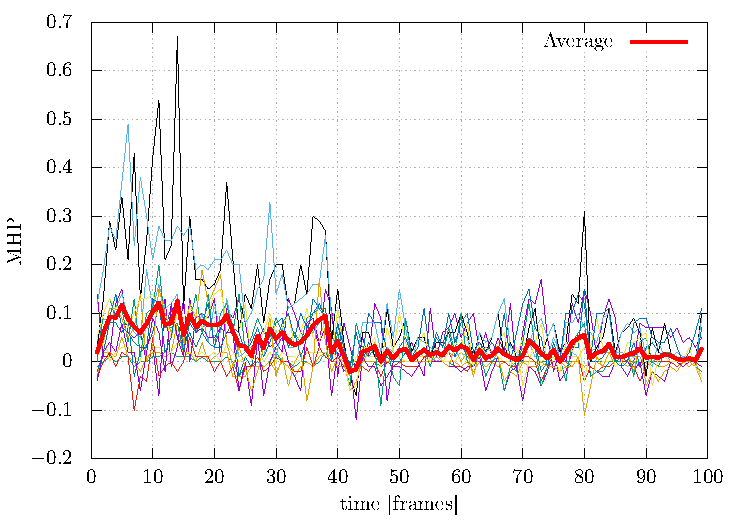
\includegraphics[scale=0.75]{PRO22_graph.pdf}
	\end{figure}
\end{frame}
\begin{frame}{MHP Change Over Time}
	\centering
	\begin{figure}[h!]
		\caption{MHP change over time for LYS-3}
		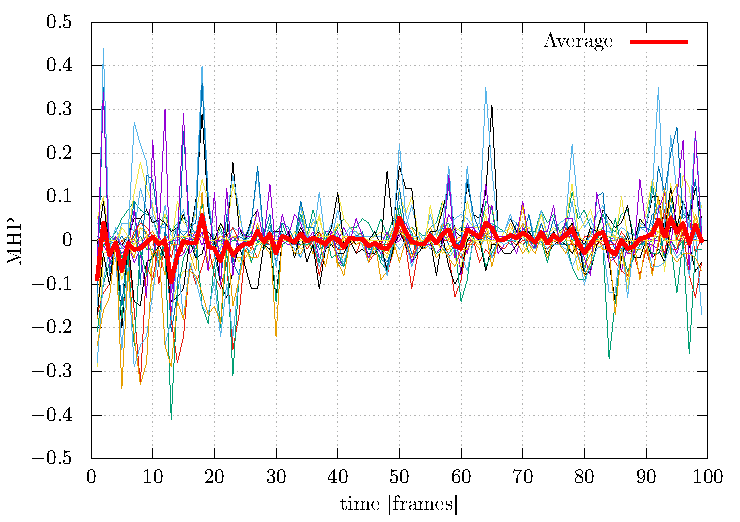
\includegraphics[scale=0.75]{LYS03_graph.pdf}
	\end{figure}
\end{frame}
\begin{frame}{MHP Change Over Time}
	\begin{itemize}
        \setlength\itemsep{1.5em}
		\uncover<2->{\item The validation shows a reasonable qualitative correlation to real data.}
		\uncover<3->{\item Performed in water (with structural optimization), the results became more accurate.}
		\uncover<4->{\item The environment did not match experiments, which could affect the accuracy.}
		\uncover<5->{\item Amino acids are small molecules, each error becomes more significant.}
		\uncover<6->{\item Larger trajectories will sample conformational space better.}
	\end{itemize}
\end{frame}

\section*{References}
\begin{frame}{References}
\end{frame}

\section*{Thankyou}
\begin{frame}
\end{frame}

\end{document}
